\documentclass[a4paper,14pt]{extreport}

% ==================================================
% КОМПИЛЯТОР: XeLaTeX
% ==================================================

\usepackage{polyglossia}
\setdefaultlanguage{russian}
\setotherlanguage{english}


\usepackage{fontspec}
\defaultfontfeatures{Ligatures=TeX}

% Установка Times New Roman для всех типов текста
\setmainfont{Times New Roman}[Script=Cyrillic]
\setsansfont{Arial}[Script=Cyrillic]
\setmonofont{Courier New}[Script=Cyrillic] % Исправляет ошибку polyglossia

% Принудительно используем Times New Roman для заголовков
\newfontfamily\cyrillicfont{Times New Roman}[Script=Cyrillic]
\newfontfamily\cyrillicfonttt{Courier New}[Script=Cyrillic]

% -------------------------------
% Геометрия страницы (стр. 12 методички)
% -------------------------------
\usepackage[
left=30mm,
right=15mm,
top=20mm,    
bottom=20mm,
footskip=10mm,
nomarginpar % Отключаем поля для заметок, чтобы не мешали рамке
]{geometry}

% -------------------------------
% Отрисовка РАМКИ (стр. 12 методички)
% -------------------------------
\usepackage{tikz}
\usetikzlibrary{calc}
\usepackage{atbegshi}


% -------------------------------
% Интервалы и абзацы
% -------------------------------
\usepackage{setspace}
\setstretch{1.5} % Межстрочный интервал 1.5 (даст примерно 30 строк)

\setlength{\parindent}{1.25cm} % Абзацный отступ (5 знаков)
\setlength{\parskip}{0pt}

% -------------------------------
% Заголовки (стр. 12-13 методички)
% -------------------------------
\usepackage[tiny,center,uppercase]{titlesec}

% Настройка для ГЛАВ (ГЛАВА 1)
\titleformat{\chapter}[block]
{\centering\bfseries\normalsize}
{\MakeUppercase{\chaptertitlename} \thechapter}
{1em}
{\MakeUppercase}

% Отступы для глав: сверху 0, после заголовка 3 интервала (ок. 18-20 пт)
\titlespacing*{\chapter}{0pt}{0pt}{20pt}

% Настройка для ПАРАГРАФОВ (1.1)
\titleformat{\section}[block]
{\bfseries\normalsize}
{\thesection}
{1em}
{}
\titlespacing*{\section}{\parindent}{12pt}{12pt}

% Команда для элементов БЕЗ нумерации (ВВЕДЕНИЕ, ЗАКЛЮЧЕНИЕ)
% Они должны быть ПРОПИСНЫМИ, по центру и начинаться с новой страницы
\newcommand{\specialchapter}[1]{%
	\clearpage
	\begin{center}
		\bfseries\MakeUppercase{#1}
	\end{center}
	\addcontentsline{toc}{chapter}{\MakeUppercase{#1}}
	\vspace{20pt}
}

% -------------------------------
% Нумерация страниц
% -------------------------------
\usepackage{fancyhdr}
\pagestyle{fancy}
\fancyhf{}
\fancyfoot[C]{\thepage} % Номер внизу по центру
\renewcommand{\headrulewidth}{0pt} % Убираем линейку сверху


% -------------------------------
% Математика
% -------------------------------
\usepackage{amsmath, amssymb}

\setlength{\abovedisplayskip}{10pt}
\setlength{\belowdisplayskip}{10pt}


% -------------------------------
% Изображения
% -------------------------------
\usepackage{graphicx}    % для вставки картинок
\usepackage{subcaption}  % для подписи под подрисунками
\usepackage{multirow} % вставить в преамбулу
\usepackage{adjustbox} % для масштабирования таблицы
\usepackage{float} 
\usepackage{url}

\usepackage{caption}

% Настройка подписей для рисунков
\captionsetup[figure]{
	name=Рисунок,
	labelsep=period,         % Заменяет двоеточие на точку: "Рисунок 1. "
	justification=centering, % Выравнивание всей надписи по центру
	singlelinecheck=false,   % Принудительно центрировать, даже если подпись короткая
	position=bottom,         % Указывает, что подпись снизу
	skip=10pt                % Отступ между картинкой и подписью
}

% Настройка отступов для плавающих объектов (рисунков [H])
\setlength{\intextsep}{20pt} % Отступ сверху и снизу рисунка от текста

\usepackage{caption}

% Общие настройки для таблиц
\captionsetup[table]{
	name=Таблица,
	labelsep=period,         % Заменяет двоеточие на точку: "Таблица 1. "
	justification=centering, % Центрирование заголовка
	singlelinecheck=false,   % Центрировать даже короткие строки
	position=top,            % Подпись над таблицей
	skip=10pt                % Отступ между подписью и таблицей
}

% -------------------------------
% Код для приложения
% -------------------------------
\usepackage{listings}
\usepackage{xcolor}

\definecolor{codebg}{RGB}{245,245,244}
\definecolor{codegreen}{RGB}{34,139,34}
\definecolor{codeblue}{RGB}{0,0,180}
\definecolor{codegray}{RGB}{120,120,120}
\definecolor{codered}{RGB}{180,0,0}

\lstdefinestyle{modern}{
	inputencoding=utf8,
	extendedchars=true,
	backgroundcolor=\color{gray!8},
	basicstyle=\ttfamily\small,
	keywordstyle=\color{purple}\bfseries,
	commentstyle=\color{teal},
	stringstyle=\color{orange},
	numbers=left,
	numberstyle=\tiny\color{gray},
	frame=none,
	rulecolor=\color{gray!40},
	breaklines=true,
	columns=fullflexible
}
\lstset{style=modern}

% -------------------------------
% Оглавление
% -------------------------------
\usepackage{tocloft}
\usepackage{ragged2e}

\renewcommand{\cftchappresnum}{ГЛАВА~}
\renewcommand{\cftchapnumwidth}{6em}

\usepackage{url}


% -------------------------------
% Оглавление (настройка через tocloft)
% -------------------------------
\usepackage{tocloft}

% 1. Настройка шрифта заголовка: normalsize (14pt), жирный, прописные
\renewcommand{\cfttoctitlefont}{\hspace*{\fill}\bfseries\normalsize\MakeUppercase}
\renewcommand{\cftaftertoctitle}{\hspace*{\fill}}

% 2. Отступы заголовка (соответствуют вашим \titlespacing для глав)
\setlength{\cftbeforetoctitleskip}{0pt}
\setlength{\cftaftertoctitleskip}{20pt} 

% 3. Настройка оформления строк в самом оглавлении
\renewcommand{\cftchappresnum}{ГЛАВА~}
\renewcommand{\cftchapnumwidth}{6em}
\renewcommand{\cftchapfont}{\normalfont} % Названия глав в списке обычным шрифтом (если нужно)
\renewcommand{\cftchappagefont}{\normalfont} % Номера страниц обычным шрифтом

% -------------------------------
% Настройка точек (отточий)
% -------------------------------
% Для глав (CHAPTER)
\renewcommand{\cftchapleader}{\cftdotfill{\cftdotsep}} 

% Для подразделов (SECTION), если они вдруг пропали
\renewcommand{\cftsecleader}{\cftdotfill{\cftdotsep}}

% Можно настроить плотность точек (опционально)
% \renewcommand{\cftdotsep}{1} % Чем меньше число, тем гуще точки

% Название
\addto\captionsrussian{%
	\renewcommand{\contentsname}{Содержание} % Пишем строчными, \MakeUppercase сделает их заглавными
}

\usepackage{longtable}
\usepackage{rotating} % для rotatebox
\usepackage{comment}

% Настройка для ОБЫЧНЫХ ПАРАГРАФОВ (слева, с отступом)
\titleformat{\section}[block]
{\bfseries\normalsize}
{\thesection}
{1em}
{}
\titlespacing*{\section}{\parindent}{12pt}{12pt}

% Команда для ЦЕНТРИРОВАННОГО НУМЕРОВАННОГО заголовка
\newcommand{\sectionc}[1]{%
	\refstepcounter{section} % Увеличиваем номер раздела
	\vspace{12pt} % Отступ сверху
	\begin{center}
		\bfseries\normalsize \thesection\quad #1 % Номер и название
	\end{center}
	\addcontentsline{toc}{section}{\protect\numberline{\thesection}#1} % Добавляем в оглавление
	\vspace{12pt} % Отступ снизу
}

% ==================================================
% ДОКУМЕНТ
% ==================================================
\begin{document}
	
	% -------------------------------
	% Нумерация страниц
	% -------------------------------
	\pagenumbering{arabic}
	\setcounter{page}{1}
	
	\addto\captionsrussian{%
		\renewcommand{\bibname}{СПИСОК ЛИТЕРАТУРЫ}%
	}
	
	% ===============================
	% ТИТУЛЬНЫЙ ЛИСТ
	% ===============================
	\begin{titlepage}
		\thispagestyle{empty}
		\singlespacing
		
		\begin{center}
			{\bfseries
				\MakeUppercase{Московский государственный университет}\\
				\MakeUppercase{имени М.В.\,Ломоносова}
				
				\vspace{0.6\baselineskip}
				ФИЛИАЛ В ГОРОДЕ ДУШАНБЕ
				
				\vspace{2\baselineskip}
				Естественно-научный факультет\\
				направление подготовки 01.03.02 Прикладная математика и информатика
			}
			
			\vspace{1.5\baselineskip}
			% Вставьте логотип. Если файла нет, закомментируйте строку ниже знаком %
			
\includegraphics[width=4cm]{Logo1.png} 
			
			\vspace{1.5\baselineskip}
			\textbf{\MakeUppercase{ОТЧЁТ
					О ПРОХОЖДЕНИИ ПРЕДДИПЛОМНОЙ  ПРАКТИКИ}}
			
			\vspace{\baselineskip}
			 {с 4 мая по 16 мая 2026 года}
		\end{center}
		
		\vspace{2\baselineskip}
		
		\hfill
		\begin{minipage}{0.6\textwidth}
			\justifying
			\setlength{\parindent}{0pt}
			\textbf{Выполнил:}\par
			студент 4 курса естественно-научного факультета направления подготовки 01.03.02~Прикладная математика и информатика\par
			Хайбулоев Дамир\,Ахлидинович
			
			\vspace{\baselineskip}
			
			\textbf{Руководитель практики от Организации:}\par
			Руководитель отдела разработки\par
			Изатшоев О. А.
			
			\vspace{\baselineskip}
			
			\textbf{Руководитель практики от Филиала:}\par
			к.ф.-м.н., доцент, зав. кафедрой математики и естественных наук\par
		Одинабеков Джасур Музофирович
		\end{minipage}
		
		\vfill
		
		\begin{center}
			Душанбе – 2026
		\end{center}
	\end{titlepage}
	
	\clearpage
	\setcounter{page}{2}
	
	\tableofcontents
	\thispagestyle{plain}
	\newpage
	
\begin{comment}
\chapter*{Аннотация}
\addcontentsline{toc}{chapter}{Аннотация}

В отчёте представлены результаты преддипломной практики, посвящённой разработке настольного программного средства для анализа одномерного уравнения переноса, сравнения численных схем и визуального исследования их свойств. В ходе практики была решена прикладная задача, которая одновременно относится к вычислительной математике, инженерии программного обеспечения и визуализации данных: требовалось создать инструмент, позволяющий не только рассчитывать решение для набора модельных случаев, но и исследовать устойчивость, точность, сходимость, влияние дискретизации и качество пользовательских схем.

Результатом работы стало интерактивное приложение на языке Python с графическим интерфейсом на базе PyQt5. В приложении реализованы аналитические и численные методы для решения уравнения переноса, механизм выбора параметров сетки и коэффициента переноса, построение срезов и анимаций, расчёт норм ошибок, анализ числа Куранта, исследование сходимости и экспорт анимации в форматы GIF и MP4. Существенной особенностью проекта является поддержка пользовательских схем: пользователь может добавить собственную явную или неявную схему через интерфейс и сравнить её с базовыми методами, не изменяя исходный код программы.

Практическая ценность полученного результата заключается в том, что программа может использоваться как учебная лаборатория для дисциплин, связанных с математическим моделированием, численными методами и разработкой научного программного обеспечения. Приложение помогает быстро переходить от теоретической формулы к наблюдаемому поведению схемы, а значит, снижает разрыв между аналитическим материалом и компьютерным экспериментом. Документ содержит описание теоретической базы, требований к системе, архитектуры проекта, особенностей программной реализации, сценариев тестирования, результатов вычислительных экспериментов и перспектив дальнейшего развития.

\tableofcontents
\end{comment}
\chapter*{Введение}
\addcontentsline{toc}{chapter}{Введение}

Современная инженерная и научная деятельность всё в большей степени опирается на вычислительный эксперимент. Для значительного класса задач математической физики аналитическое решение либо отсутствует, либо существует только для ограниченного набора частных случаев. Поэтому качество подготовки специалиста в области прикладной математики и программной инженерии во многом определяется не только знанием теории, но и умением разрабатывать инструменты для численного исследования моделей, анализировать устойчивость алгоритмов и интерпретировать полученные результаты.

Одним из базовых объектов изучения в вычислительной математике является уравнение переноса. Оно возникает при описании конвективных процессов, движения примесей, распространения сигналов и иных явлений, в которых некоторое поле перемещается вдоль характеристик без внутреннего источника. Несмотря на простую формальную запись, эта модель демонстрирует широкий спектр методических вопросов: влияние выбора схемы на диссипацию и дисперсию, зависимость результата от числа Куранта, различие между явными и неявными подходами, роль искусственной вязкости, чувствительность к разрывным и гладким начальным данным.

Для эффективного изучения указанных аспектов недостаточно иметь набор отдельных скриптов. Требуется программное средство, которое объединяет построение аналитического решения, набор типовых разностных схем, расчёт ошибок и удобную визуализацию. Особенно важна возможность быстро переключаться между режимами коэффициента переноса $a$, изменять сеточные параметры, сравнивать несколько методов на одном графике и отслеживать эволюцию решения во времени. Такие функции превращают программу в лабораторию численного анализа, пригодную и для индивидуального исследования, и для учебного процесса.

Целью преддипломной практики являлась разработка настольного приложения для исследования численных схем решения одномерного уравнения переноса с акцентом на воспроизводимость вычислительных экспериментов, удобство интерфейса и расширяемость архитектуры. Для достижения цели были поставлены следующие задачи:

\begin{enumerate}
    \item изучить математическую постановку задачи и выделить те случаи, для которых возможно построение аналитического эталона;
    \item определить перечень численных схем, которые должны войти в базовую поставку приложения;
    \item сформулировать функциональные и нефункциональные требования к интерфейсу и вычислительному модулю;
    \item реализовать механизм параметризации коэффициента переноса и начального условия;
    \item реализовать набор методов анализа качества решения: нормы ошибок, анализ сходимости, расчёт CFL-числа, экспорт графических результатов;
    \item провести вычислительные эксперименты и подготовить документированное описание полученного результата.
\end{enumerate}

Объектом исследования является процесс численного решения одномерного уравнения переноса, а предметом исследования выступают алгоритмы и программные средства, обеспечивающие его интерактивное изучение в настольном приложении. Практическая значимость работы состоит в создании инструмента, который может быть использован как элемент учебно-методического обеспечения, как основа для выпускной квалификационной работы и как стартовая платформа для дальнейшего расширения функциональности в сторону более сложных моделей.

\chapter{Цели, задачи и содержание преддипломной практики}

Преддипломная практика является завершающим этапом подготовки выпускника, на котором проверяется способность применять накопленные знания в рамках цельного инженерного проекта. В отличие от учебной или производственной практики, на данном этапе акцент смещается на самостоятельную постановку технических решений, обоснование выбранных архитектурных и алгоритмических подходов, а также на формирование результатов, которые могут быть непосредственно использованы в дипломном проектировании.

В рамках рассматриваемой работы преддипломная практика была организована как последовательность взаимосвязанных этапов. На первом этапе была выполнена аналитическая проработка предметной области. Необходимо было сопоставить математическое содержание уравнения переноса с требованиями к программному продукту. Выяснилось, что для учебно -- исследовательского приложения принципиально важно поддержать не один, а несколько режимов задания коэффициента $a$: постоянный коэффициент, зависимость от пространственной переменной, зависимость от времени и смешанную зависимость от $x$ и $t$. Это позволяет охватить разные классы задач и демонстрирует особенности поведения схем на существенно различных постановках.

На втором этапе была сформирована концепция программного продукта. Приложение должно было выполнять сразу несколько ролей: служить калькулятором аналитического решения, инструментом сравнения численных методов, средством визуального анализа и платформой для пользовательских экспериментов. Следовательно, система должна быть интерактивной, расширяемой и устойчивой к некорректному вводу. Из этого напрямую следовали требования к выбору технологий: язык разработки должен иметь сильную экосистему для численных расчётов и интерфейсов, а графическая библиотека обязана обеспечивать построение интерактивных визуализаций.

На третьем этапе была выполнена детальная проработка алгоритмов. Помимо реализации классических явных схем против потока, Лакса -- Фридрихса, Лакса -- Вендроффа и Мак -- Кормака, в проект были включены TVD- и MUSCL-подходы, варианты с искусственной вязкостью, а также ряд неявных схем, включая центральные, апвиндные и регуляризованные методы. Отдельной задачей стало внедрение настраиваемых пользовательских схем, задаваемых формульно. Это требовало разработки формата хранения, валидации, интерпретации выражений и согласования их с общим вычислительным контуром.

На четвёртом этапе выполнялась разработка интерфейса. Необходимо было организовать экран так, чтобы пользователь мог за один сеанс работы изменить тип коэффициента переноса, диапазоны сетки, число узлов, набор сравниваемых схем, режим отображения аналитического решения и параметры визуального окна. Параллельно была предусмотрена область текстового вывода, в которую помещаются отчёты о расчёте, ошибки, предупреждения и краткие итоги анализа.

На заключительных этапах практика была направлена на отладку, тестирование и подготовку документации. Были проверены типовые сценарии, оценены узкие места, внесены коррективы в обработку ошибок и механизм экспорта анимаций. Итогом стала программная система, которая демонстрирует полноценный цикл разработки: от математической постановки и алгоритмизации до пользовательского интерфейса и описания результатов.

Содержательно практика позволила закрепить и объединить знания по следующим направлениям:

\begin{itemize}
    \item математическое моделирование и постановка задачи переноса;
    \item численные методы решения задач математической физики;
    \item программирование на Python и работа с научными библиотеками;
    \item проектирование графических пользовательских интерфейсов;
    \item сериализация пользовательских данных и обеспечение расширяемости системы;
    \item визуальный анализ данных и подготовка отчётной документации.
\end{itemize}

Таким образом, преддипломная практика не свелась к написанию отдельного скрипта, а представляла собой инженерную работу по созданию законченного программного продукта, ориентированного на решение учебно-исследовательских задач в области численного анализа.

\chapter{Теоретические основы решения уравнения переноса}

\sectionc{Математическая постановка задачи}

В базовом виде одномерное уравнение переноса можно записать как

\begin{equation}
    \frac{\partial u}{\partial t} + a(x,t) \frac{\partial u}{\partial x} = 0,
\end{equation}

где $u(x,t)$ --- искомая функция, а $a(x,t)$ --- скорость переноса, которая в зависимости от постановки может быть постоянной или переменной. Начальное условие задаётся функцией

\begin{equation}
    u(x,0) = \varphi_0(x).
\end{equation}

Смысл уравнения состоит в том, что профиль $u$ переносится вдоль характеристик, причём форма решения в простейших случаях сохраняется. Именно это делает задачу удобной для учебного анализа: с одной стороны, модель достаточно проста для построения аналитических эталонов, с другой --- она чувствительна к дискретизации и позволяет наглядно увидеть особенности различных разностных схем.

Если коэффициент переноса постоянен, то решение имеет вид

\begin{equation}
    u(x,t) = \varphi_0(x - at).
\end{equation}

То есть начальный профиль просто смещается без изменения формы. Однако при численном решении реальное поведение зависит от выбранной схемы: одни методы искусственно сглаживают профиль, другие создают паразитические колебания, третьи дают приемлемый баланс между устойчивостью и точностью. Поэтому уравнение переноса является классическим тестом для сравнения численных методов.

\sectionc{Метод характеристик}

Для аналитического исследования задачи переноса ключевым инструментом является метод характеристик. Идея метода состоит в поиске кривых $x(t)$ в плоскости переменных, вдоль которых значение решения сохраняется или изменяется по упрощённому закону. Для рассматриваемой модели характеристические уравнения принимают вид

\begin{equation}
    \frac{dx}{dt} = a(x,t), \qquad \frac{du}{dt} = 0.
\end{equation}

Второе соотношение означает, что вдоль характеристики величина $u$ постоянна. Следовательно, если известна точка пересечения характеристики с начальной линией $t=0$, то значение решения в любой последующей точке определяется начальным условием. Отсюда возникает общая идея аналитического решения: найти отображение, которое каждой точке $(x,t)$ ставит в соответствие начальную координату $\xi$, и затем вычислить

\begin{equation}
    u(x,t) = \varphi_0(\xi(x,t)).
\end{equation}

В разработанном приложении эта идея использована как для прямого вычисления аналитического решения, так и для визуализации характеристик. Для случая переменного коэффициента транспортировки аналитические выражения определены для нескольких типовых зависимостей: $a=a(x)$, $a=a(t)$ и ряда каталогизированных случаев $a=a(x,t)$. Таким образом, интерфейс не ограничивается только постоянной скоростью переноса и позволяет демонстрировать более содержательные сценарии.

\sectionc{Типовые случаи коэффициента переноса}

Для зависимости $a=a(x)$ характеристическое описание можно выразить через интеграл

\begin{equation}
    F(x) = \int \frac{dx}{a(x)}.
\end{equation}

Тогда координата начальной точки восстанавливается по соотношению $F(\xi)=F(x)-t$. В программной реализации эта идея реализуется через численное интегрирование. Это позволяет обойтись без символьного вывода замкнутой формулы, сохраняя при этом связь с характеристическим подходом.

Для зависимости $a=a(t)$ характерен другой тип преобразования. Пусть

\begin{equation}
    S(t)=\int_0^t a(\tau)\,d\tau.
\end{equation}

Тогда аналитическое решение запишется как

\begin{equation}
    u(x,t)=\varphi_0(x-S(t)).
\end{equation}

Наконец, для каталога функций $a(x,t)$ в программе предусмотрены специально подготовленные случаи, например $a=x-t$, $a=x+t$, $a=x\,t$, $a=x\exp(-t)$ и аффинные комбинации вида $a=\alpha x+\beta t+d$. Для них построены формулы, позволяющие получать эталонное решение и сравнивать его с численными результатами.

Поддержка этих вариантов имеет важное методическое значение. Пользователь может увидеть, что даже при сохранении общей структуры уравнения свойства решения и требования к сетке меняются. Следовательно, приложение позволяет изучать не только отдельный метод, но и его поведение на семействах задач.

\sectionc{Разностные схемы и дискретизация}

Пусть пространство и время дискретизированы равномерными сетками

\begin{equation}
    x_i = x_{\min} + i h, \qquad t^n = t_{\min} + n\tau,
\end{equation}

где $h$ --- пространственный шаг, $\tau$ --- временной шаг. Тогда численное решение обозначается через $u_i^n \approx u(x_i,t^n)$. Для уравнения переноса естественным является введение безразмерного параметра

\begin{equation}
    \lambda_i^n = \frac{a_i^n\tau}{h},
\end{equation}

который характеризует относительное смещение информации за один временной шаг.

В приложении реализованы следующие основные группы схем:

\begin{itemize}
    \item явные апвиндные и центральные схемы;
    \item явные схемы второго порядка, включая Лакса -- Вендроффа и Мак -- Кормака;
    \item TVD- и MUSCL-подходы с ограничителями потоков;
    \item схемы с искусственной линейной и нелинейной вязкостью;
    \item неявные трёхдиагональные и пентадиагональные схемы;
    \item пользовательские схемы, заданные формулами для обновления узлов или коэффициентов матрицы.
\end{itemize}

Явная схема против потока для $a>0$ имеет вид

\begin{equation}
    u_i^{n+1}=u_i^n-\lambda_i^n\left(u_i^n-u_{i-1}^n\right).
\end{equation}

Она проста и надёжна, но обладает численной вязкостью, сглаживающей решение. Схема Лакса--Фридрихса заменяет центральную производную на комбинацию усреднения и разности:

\begin{equation}
    u_i^{n+1}=\frac{u_{i+1}^n+u_{i-1}^n}{2}-\frac{\lambda_i^n}{2}(u_{i+1}^n-u_{i-1}^n).
\end{equation}

Схема Лакса--Вендроффа повышает порядок аппроксимации за счёт добавления второго разностного члена:

\begin{equation}
    u_i^{n+1}=u_i^n-\frac{\lambda_i^n}{2}(u_{i+1}^n-u_{i-1}^n)+\frac{(\lambda_i^n)^2}{2}(u_{i+1}^n-2u_i^n+u_{i-1}^n).
\end{equation}

С ростом порядка точности растёт и чувствительность к разрывам и крутым фронтам. Именно поэтому в реальных вычислительных экспериментах востребованы TVD- и MUSCL-подходы, которые подавляют нефизические осцилляции с помощью ограничителей. В проекте реализованы варианты с ограничителями minmod и MC, что даёт возможность исследовать компромисс между монотонностью и точностью.

\sectionc{Неявные методы и решение систем линейных уравнений}

Неявные схемы требуют решения линейной системы на каждом временном шаге. Их основное преимущество состоит в большей устойчивости, особенно при сравнительно крупных временных шагах. Цена за это --- увеличение вычислительных затрат и необходимость организовать надёжный решатель для ленточных матриц.

В разработанном приложении применяются два подхода. Первый связан с использованием трёхдиагональной структуры, для которой реализован метод прогонки. Второй подход опирается на матричное описание пользовательской схемы и использует решатель для ленточных систем из библиотеки SciPy. Такое разделение позволяет с одной стороны эффективно вычислять стандартные схемы, а с другой --- дать пользователю гибкий механизм задания собственной матрицы.

С инженерной точки зрения это важный архитектурный выбор. Если все схемы реализовать в одном стиле, код будет менее гибким. Если же допустить несколько форматов схем и унифицировать их через общую функцию разрешения имени метода, можно сохранить расширяемость без усложнения интерфейса пользователя. Именно такой подход реализован в проекте.

\sectionc{Устойчивость, число Куранта и нормы ошибок}

Для гиперболических задач важнейшей характеристикой является число Куранта--Фридрихса--Леви:

\begin{equation}
    \mathrm{CFL}=\max_{x,t}\left|a(x,t)\right|\frac{\tau}{h}.
\end{equation}

Если значение CFL слишком велико, многие явные схемы становятся неустойчивыми. В приложении предусмотрен специальный инструмент, вычисляющий число CFL по заданной сетке и параметрам коэффициента. Пользователь получает не только численное значение, но и краткую интерпретацию, позволяющую быстро определить потенциальный риск потери устойчивости.

Для оценки точности численного решения реализован расчёт норм ошибок относительно аналитического эталона. Используются нормы

\begin{align}
    \|e\|_{L_1} &= h \sum_i |u_i-\tilde{u}_i|, \\
    \|e\|_{L_2} &= \left(h \sum_i (u_i-\tilde{u}_i)^2\right)^{1/2}, \\
    \|e\|_{L_\infty} &= \max_i |u_i-\tilde{u}_i|,
\end{align}
где $\tilde{u}_i$ обозначает аналитическое решение. Одновременный анализ нескольких норм даёт более полную картину. Например, схема может демонстрировать умеренную ошибку в $L_2$, но иметь заметные локальные выбросы в $L_\infty$. В контексте учебного исследования это особенно полезно, поскольку позволяет обсуждать не только среднюю точность, но и поведение схемы в критических точках.

\chapter{Требования к программной системе}

\sectionc{Функциональные требования}

После анализа предметной области были сформулированы требования к разрабатываемому приложению. В первую очередь система должна обеспечивать полный цикл исследования: от задания параметров модели до получения визуальных и численных выводов. Это означает, что графический интерфейс не может ограничиваться одной кнопкой расчёта; он обязан поддерживать интерактивный сценарий работы с множеством параметров и режимов отображения.

К основным функциональным требованиям относятся:

\begin{longtable}{p{0.08\textwidth}p{0.35\textwidth}p{0.47\textwidth}}
№ & Требование & Содержание \\
1 & Задание модели & Выбор режима коэффициента переноса: постоянный, зависящий от $x$, зависящий от $t$, либо выбираемый из каталога $a(x,t)$. \\
2 & Задание начального условия & Ввод аналитического выражения $\varphi_0(x)$ с последующим преобразованием к вычислимой функции. \\
3 & Настройка сетки & Ввод границ области по пространству и времени, а также количества узлов по каждой координате. \\
4 & Выбор схем & Отметка одной или нескольких встроенных или пользовательских схем для одновременного сравнения. \\
5 & Визуализация & Построение анимации, срезов, контурных и трёхмерных графиков. \\
6 & Анализ ошибок & Расчёт норм ошибок, формирование таблиц итоговых значений, визуализация динамики норм. \\
7 & Анализ сходимости & Построение графика зависимости ошибки от шага сетки для выбранной схемы. \\
8 & Расчёт CFL & Определение числа Куранта и выдача краткой оценки устойчивости. \\
9 & Работа с пользовательскими схемами & Добавление, удаление, сохранение и повторная загрузка собственных схем пользователя. \\
10 & Экспорт результатов & Сохранение анимации в форматах GIF и MP4 с индикацией прогресса. \\
\end{longtable}

Следует отметить, что требования к пользовательским схемам были сформулированы отдельно. Пользователь должен иметь возможность задать либо явную формулу перехода на новый слой, либо неявную схему через описание правой части и коэффициентов матрицы. Такое решение существенно расширяет образовательный потенциал системы: приложение превращается из статичного демонстратора в площадку для постановки собственных вычислительных экспериментов.

\sectionc{Нефункциональные требования}

Нефункциональные требования в рассматриваемом проекте не менее важны, чем функциональные. Система ориентирована на учебную и исследовательскую работу, поэтому ошибки ввода, зависания интерфейса или невозможность повторить эксперимент снижают ценность продукта даже при корректно реализованных формулах. По этой причине были выделены следующие нефункциональные требования:

\begin{itemize}
    \item \textbf{наглядность}: все ключевые результаты должны быть доступны в визуальной форме;
    \item \textbf{отказоустойчивость}: программа обязана корректно сообщать пользователю о некорректном вводе, а не завершаться аварийно;
    \item \textbf{расширяемость}: добавление новой схемы не должно требовать перестройки архитектуры;
    \item \textbf{повторяемость экспериментов}: пользовательские схемы и настройки должны сохраняться между запусками;
    \item \textbf{приемлемая производительность}: расчёты на сетках средней плотности должны выполняться без ощутимых задержек;
    \item \textbf{кроссплатформенность}: приложение должно запускаться в типичной настольной среде без жёсткой привязки к конкретной операционной системе.
\end{itemize}

Отдельно стоит подчеркнуть требование к объяснимости результатов. В системе присутствует текстовая область вывода, где отображаются краткие отчёты, сообщения об ошибках, итоги расчётов и список пропущенных схем. Это важная деталь пользовательского опыта, поскольку при одновременном сравнении нескольких методов пользователь должен понимать, какие вычисления завершились успешно, а какие были пропущены из-за несоответствия условий применимости.

\sectionc{Сценарии использования}

Для оценки полноты требований были выделены типовые сценарии использования:

\begin{enumerate}
    \item студент выбирает начальное условие $\varphi_0(x)=\exp(-x^2)$, включает несколько схем и сравнивает их на одном графике;
    \item преподаватель демонстрирует влияние CFL-числа на устойчивость явной схемы, последовательно изменяя сеточные параметры;
    \item исследователь добавляет собственную схему через формулу, сохраняет её в конфигурацию и сопоставляет с базовыми методами;
    \item пользователь экспортирует анимацию эволюции решения для включения в презентацию или отчёт;
    \item разработчик проверяет порядок сходимости выбранной схемы, последовательно уточняя сетку и анализируя логарифмический график ошибки.
\end{enumerate}

Эти сценарии напрямую определили состав интерфейса и логику взаимодействия между вычислительным ядром и средствами визуализации.

\chapter{Проектирование архитектуры приложения}

\sectionc{Выбор технологического стека}

В качестве языка реализации выбран Python. Такое решение обусловлено несколькими факторами. Во-первых, Python является фактическим стандартом для быстрого прототипирования вычислительных приложений и учебных научных систем. Во-вторых, экосистема языка включает библиотеки NumPy, SciPy и SymPy, которые покрывают основные вычислительные потребности проекта: векторные операции, численное интегрирование, решение систем линейных уравнений и интерпретацию символьных выражений. В-третьих, наличие PyQt5 и Plotly позволяет совместить настольный интерфейс с современными интерактивными графиками.

Для графического интерфейса использована библиотека PyQt5. Она предоставляет зрелую модель виджетов, механизмы сигналов и слотов, а также удобные средства компоновки экранов. Важным аргументом в её пользу стало наличие диалоговых окон, списков, таблиц, полос прогресса и потоков, которые понадобились для реализации полноценного пользовательского интерфейса.

Для визуализации результатов применён Plotly. По сравнению со статическими средствами отображения он предоставляет интерактивные анимации, элементы управления воспроизведением, ползунки времени, масштабирование и экспорт в веб-представление. В контексте учебной задачи это особенно полезно: пользователь может не только посмотреть итоговый график, но и динамически исследовать эволюцию решения.

\sectionc{Логическая структура системы}

Архитектура приложения построена вокруг нескольких логических подсистем:

\begin{enumerate}
    \item \textbf{подсистема построения контекста задачи};
    \item \textbf{подсистема вычислительных схем};
    \item \textbf{подсистема анализа ошибок и сходимости};
    \item \textbf{подсистема визуализации};
    \item \textbf{подсистема работы с пользовательскими схемами};
    \item \textbf{подсистема графического интерфейса и диалогов}.
\end{enumerate}

Ключевым архитектурным объектом является контекст задачи. В нём хранятся пространственная и временная сетки, функция коэффициента переноса, функция аналитического решения, а также служебные признаки, например факт постоянства коэффициента и его численное значение. Такая инкапсуляция позволяет передавать схемам единый объект с согласованным набором данных. Следовательно, каждая схема получает одинаковый интерфейс входа и не зависит от деталей пользовательского интерфейса.

С практической точки зрения это снижает связанность модулей. Вычислительный код не знает о наличии полей ввода, кнопок и выпадающих списков; он получает только готовый контекст. Аналогично, интерфейс не содержит в себе математической логики схем, а лишь инициирует расчёт, собирает параметры и выводит результаты. Подобное разделение соответствует принципам проектирования расширяемых систем и облегчает дальнейшее развитие проекта.

\sectionc{Организация набора схем}

Встроенные схемы сгруппированы в два словаря: явные и неявные (рисунок \eqref{fig:image2026-04-2516-14-33}).

\begin{figure}[H]
	\centering
	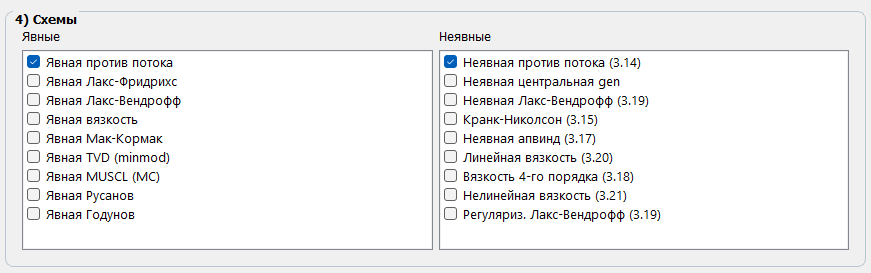
\includegraphics[width=0.8\textwidth]{image_2026-04-25_16-14-33.png}
	\caption{Группировка явных и неявных схем}
	\label{fig:image2026-04-2516-14-33}
\end{figure}

Такое решение даёт несколько преимуществ. Во-первых, интерфейс может автоматически сформировать список доступных методов без ручного дублирования имён. Во-вторых, добавление новой схемы сводится к включению функции в соответствующий словарь. В-третьих, пользователь получает естественное разделение методов по классу реализации.

Для справочного режима создан отдельный каталог текстовых формул, рисунок \eqref{fig:image2026-04-2516-19-51}. 

\begin{figure}[H]
	\centering
	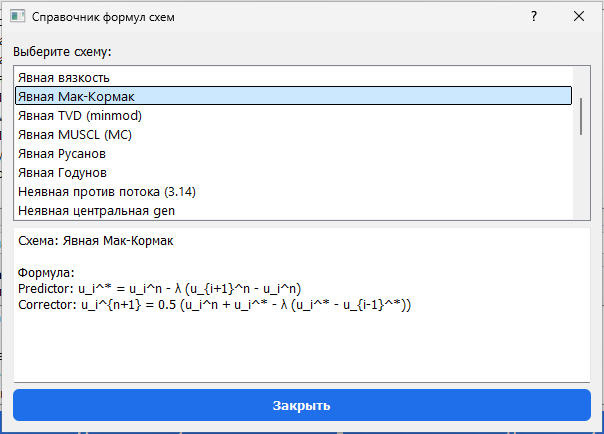
\includegraphics[width=0.8\textwidth]{image_2026-04-25_16-19-51.png}
	\caption{Справочник схем}
	\label{fig:image2026-04-2516-19-51}
\end{figure}

Он содержит компактные описания схем в математическом виде и используется в диалоговом окне справочника. Это важный элемент методической поддержки: пользователь не просто выбирает неизвестное имя алгоритма, а может быстро ознакомиться с формулой и сопоставить её с наблюдаемым поведением на графике.

\sectionc{Поддержка пользовательских схем}

Одной из наиболее значимых архитектурных особенностей проекта является механизм пользовательских схем (рисунок \eqref{fig:image2026-04-2516-22-40}). 

\begin{figure}[H]
	\centering
	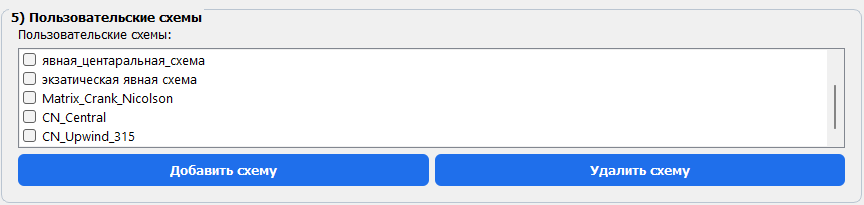
\includegraphics[width=0.7\linewidth]{image_2026-04-25_16-22-40.png}
	\caption{Интерфейс для польтзовательских схем}
	\label{fig:image2026-04-2516-22-40}
\end{figure}

Система поддерживает три типа пользовательского описания, показанных на рисунке \eqref{fig:image2026-04-2516-26-05}:

\begin{itemize}
    \item явная схема, задаваемая формулой для вычисления нового значения узла;
    \item неявная схема в режиме шаблонов, где пользователь выбирает тип матричной структуры и задаёт правую часть;
    \item матричная неявная схема, для которой пользователь непосредственно задаёт диагонали ленточной матрицы и выражение для правой части.
\end{itemize}

\begin{figure}[H]
	\centering
	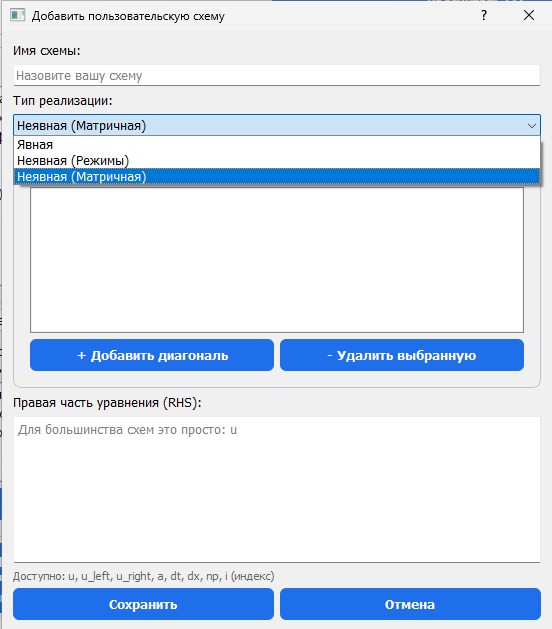
\includegraphics[width=0.7\linewidth]{image_2026-04-25_16-26-05.png}
	\caption{Режимы ввода пользовательских схем}
	\label{fig:image2026-04-2516-26-05}
\end{figure}


Данные пользовательских схем хранятся в JSON-файле. Это обеспечивает переносимость и повторяемость экспериментов. При запуске приложения схемы автоматически загружаются, а при изменении списка сохраняются обратно. В результате пользователь один раз настраивает нужный набор методов и далее может использовать его без повторного ввода.

Такой подход демонстрирует важный принцип программной инженерии: расширяемость достигается не через редактирование исходного кода, а через выделение устойчивого формата конфигурации. В данном проекте пользователь фактически получает мини-язык задания схем, встроенный в настольное приложение.

\sectionc{Интерфейс пользователя}

Экран приложения разделён на логические блоки: задание коэффициента переноса и начального условия, настройка сетки, параметры окна графика, расчёт CFL, выбор схем, список пользовательских схем, кнопки анализа и область текстового вывода. Такое разбиение позволяет последовательно пройти путь от постановки задачи к анализу результата. Интерфейс показан на рисунке \eqref{fig:graphs}

\begin{figure}[H]
	\centering
	\vspace{10pt}
	\begin{subfigure}[b]{0.45\textwidth}
		\centering
		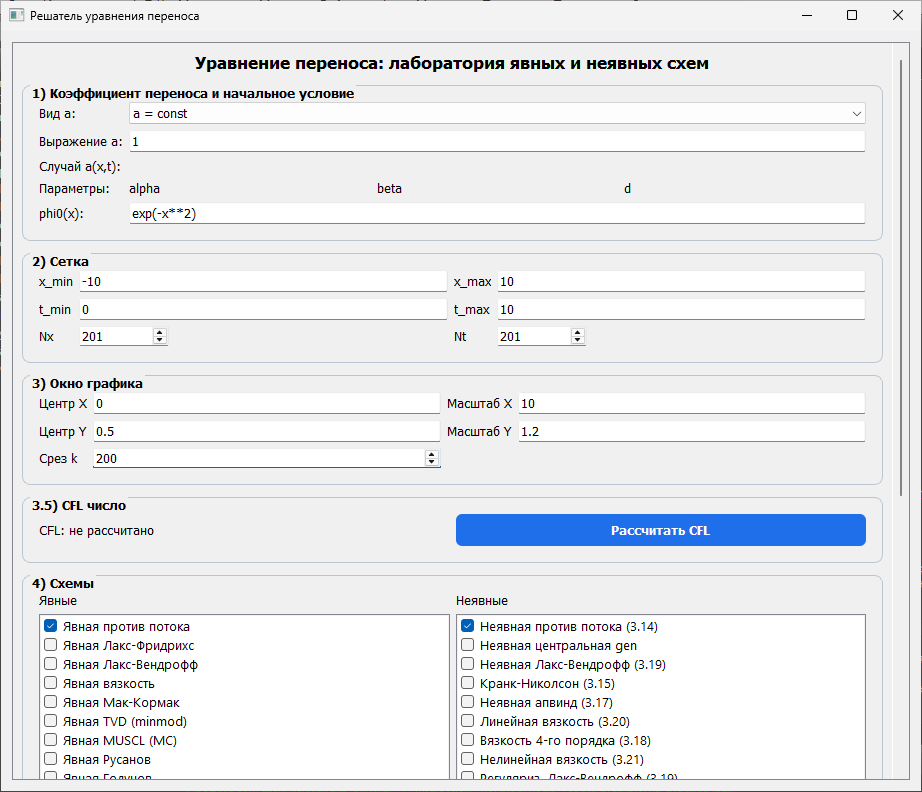
\includegraphics[width=\textwidth,height=7cm]{image_2026-04-25_16-29-08.png}
		\label{fig:graph1}
	\end{subfigure}
	\hfill
	\begin{subfigure}[b]{0.45\textwidth}
		\centering
		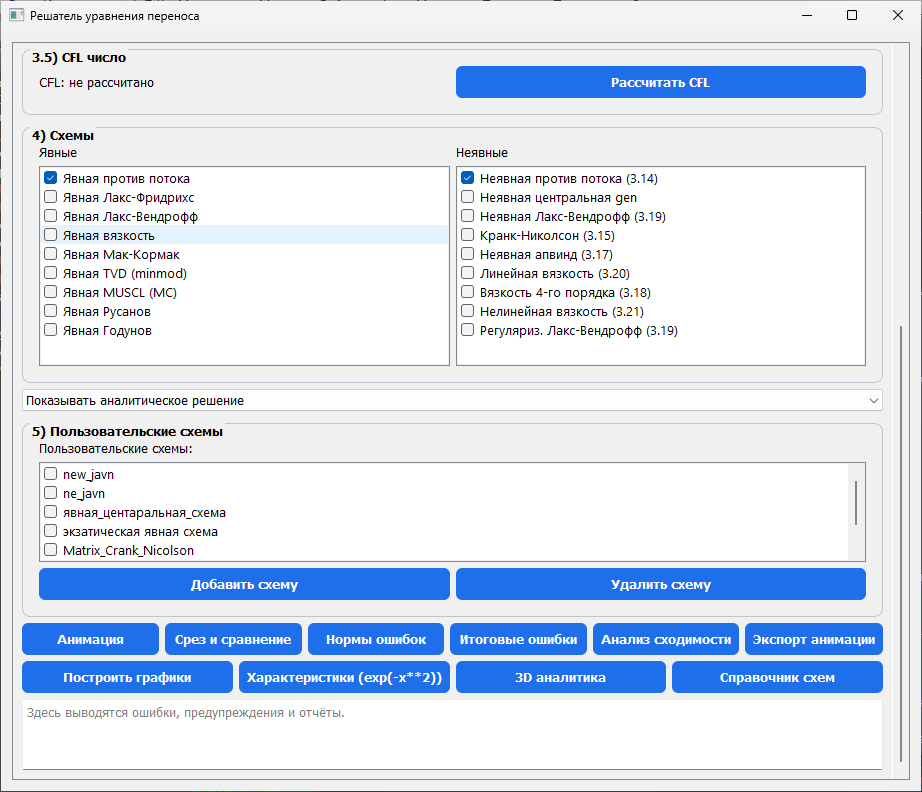
\includegraphics[width=\textwidth,height=7cm]{image_2026-04-25_16-29-36.png}
		\label{fig:graph2}
	\end{subfigure}
	
	\caption{Интерфейс программы предствленный в двух рисунках}
	\label{fig:graphs}
\end{figure}

Интерфейс ориентирован на компактность без перегрузки деталями. Большинство действий выполняется с главного окна, а дополнительные операции вынесены в отдельные диалоговые формы. Например, добавление пользовательской схемы реализовано в отдельном диалоге, а таблица итоговых норм ошибок отображается в модальном окне. Это позволяет сохранить основной экран достаточно чистым и не перегружать пользователя редкими настройками.

\chapter{Программная реализация системы}

\sectionc{Построение вычислительного контекста}

Создание контекста задачи начинается с чтения пользовательских параметров: границ по пространству и времени, числа узлов, выражения для начального условия и вида коэффициента переноса. Далее формируются равномерные сетки и строятся функции, описывающие коэффициент $a(x,t)$ и аналитическое решение $u(x,t)$. Такой подход позволяет единообразно работать как с постоянным коэффициентом, так и с более сложными зависимостями.

При интерпретации пользовательских выражений используется библиотека SymPy. Она преобразует строковую формулу в символьное выражение, после чего создаётся численная функция с использованием NumPy-модулей. Достоинство этого решения заключается в гибкости: пользователь может вводить выражения наподобие \texttt{exp(-x**2)}, \texttt{sin(x)} или комбинации с функцией \texttt{heaviside}. Недостатком является необходимость тщательно обрабатывать ошибки разбора, что и реализовано в приложении через исключения и сообщения в интерфейсе.

Для случая $a=a(x)$ программа дополнительно проверяет конечность значений, отсутствие нулей на сетке и сохранение знака коэффициента. Эти проверки принципиально важны, поскольку аналитическое представление через характеристический интеграл и обратную интерполяцию требует монотонности соответствующего преобразования. Таким образом, система предотвращает вычислительные сценарии, которые привели бы либо к некорректным результатам, либо к неочевидным сбоям.

\sectionc{Реализация явных схем}

Каждая явная схема оформлена как отдельная функция, принимающая контекст и возвращающая двумерный массив решения. Внутри временного цикла производится вычисление коэффициента Куранта и обновление внутренних узлов. Граничные значения восстанавливаются через аналитическое решение, что обеспечивает согласованность постановки и позволяет сосредоточиться на анализе внутренней аппроксимации.

Набор явных методов включает схему против потока, Лакса--Фридрихса, Лакса--Вендроффа, Мак-Кормака, варианты с искусственной вязкостью, а также TVD- и MUSCL-алгоритмы. Это делает приложение достаточно репрезентативным с методической точки зрения. Пользователь может сравнить простейший апвиндный метод, более точные схемы второго порядка и модификации, ориентированные на подавление осцилляций. Пример на рисунке \eqref{fig:image2026-04-2516-46-05}.

\begin{figure}[H]
	\centering
	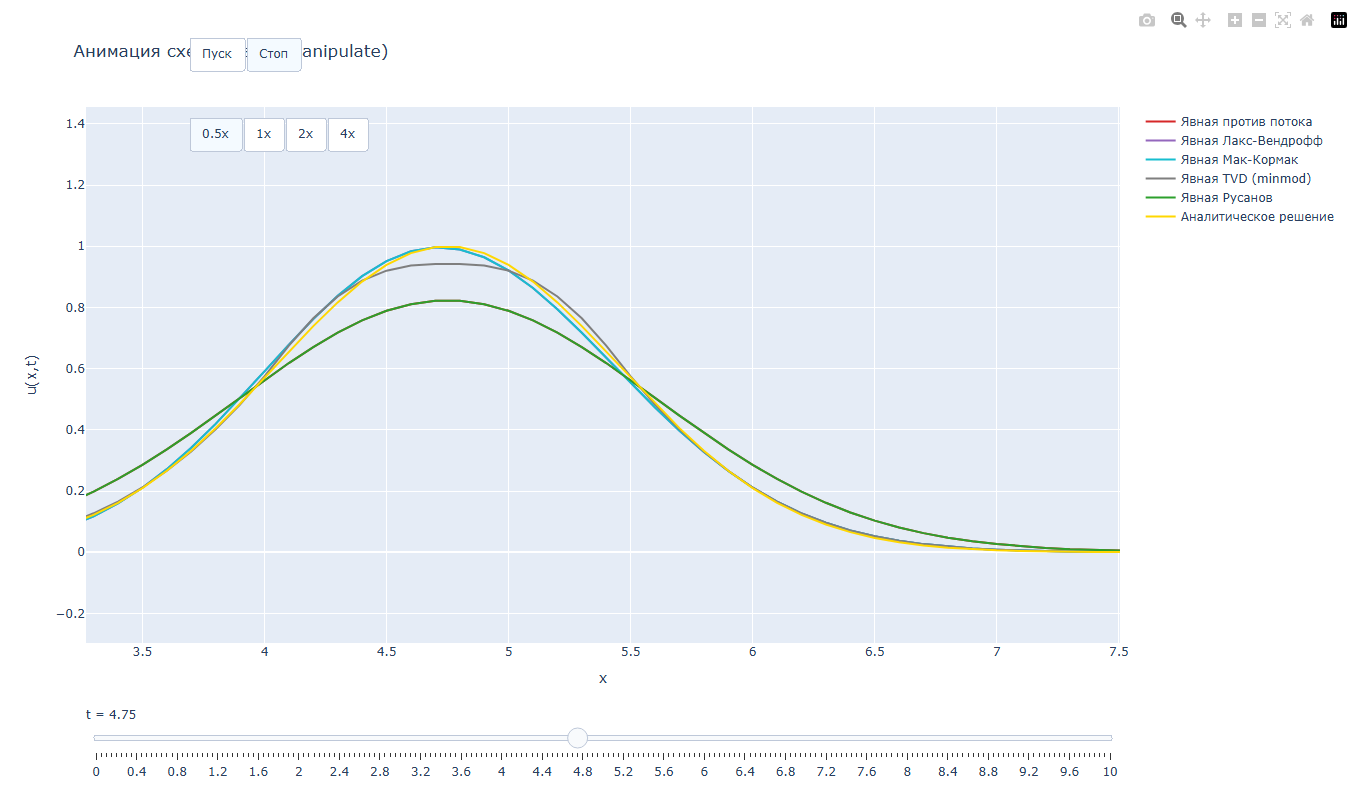
\includegraphics[width=0.9\linewidth]{image_2026-04-25_16-46-05.png}
	\caption{}
	\label{fig:image2026-04-2516-46-05}
\end{figure}


В реализации TVD- и MUSCL-подходов используются ограничители minmod и MC (рисунок  \eqref{fig:image2026-04-2516-49-52}). Для каждого узла вычисляются локальные отношения соседних разностей, после чего строится корректирующий член. Такой код несколько сложнее простых явных схем, но его включение в проект оправдано: без него приложение не давало бы возможности обсуждать современные монотонные подходы к численному решению гиперболических задач.

\begin{figure}[H]
	\centering
	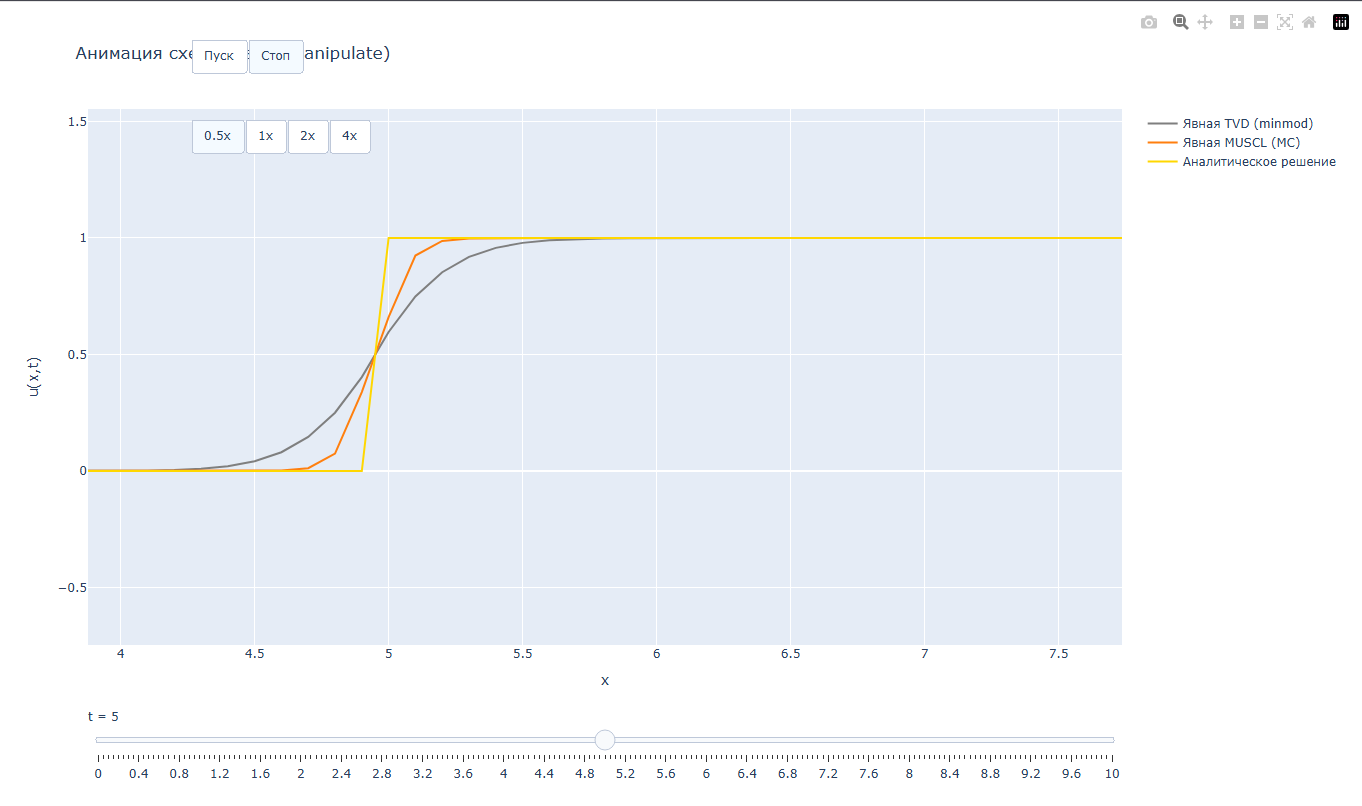
\includegraphics[width=0.9\linewidth]{image_2026-04-25_16-49-52}
	\caption{}
	\label{fig:image2026-04-2516-49-52}
\end{figure}


\sectionc{Реализация неявных схем}

Неявные схемы разделены на два класса. Первый класс состоит из стандартных схем, для которых можно заранее задать структуру трёхдиагональной системы и решить её методом прогонки. Реализация метода прогонки выделена в отдельную функцию, принимающую поддиагональ, диагональ, наддиагональ и правую часть. Такая декомпозиция делает код повторно используемым и упрощает сопровождение.

Второй класс связан с пользовательскими матричными схемами. В этом случае из пользовательского описания извлекается набор диагоналей ленточной матрицы и формула правой части, после чего система собирается на каждом временном шаге и передаётся решателю \texttt{solve\_banded} из SciPy. Поддержка ленточной матрицы особенно полезна, поскольку многие практические схемы имеют именно такую структуру, а её хранение в плотном виде было бы избыточным.

Программно важно, что и стандартные, и пользовательские неявные схемы возвращают результат в одном и том же формате. Как на рисунке \eqref{fig:image2026-04-2516-55-57}, здесь схема \text{CN Central} является пользовательской.

\begin{figure}[H]
	\centering
	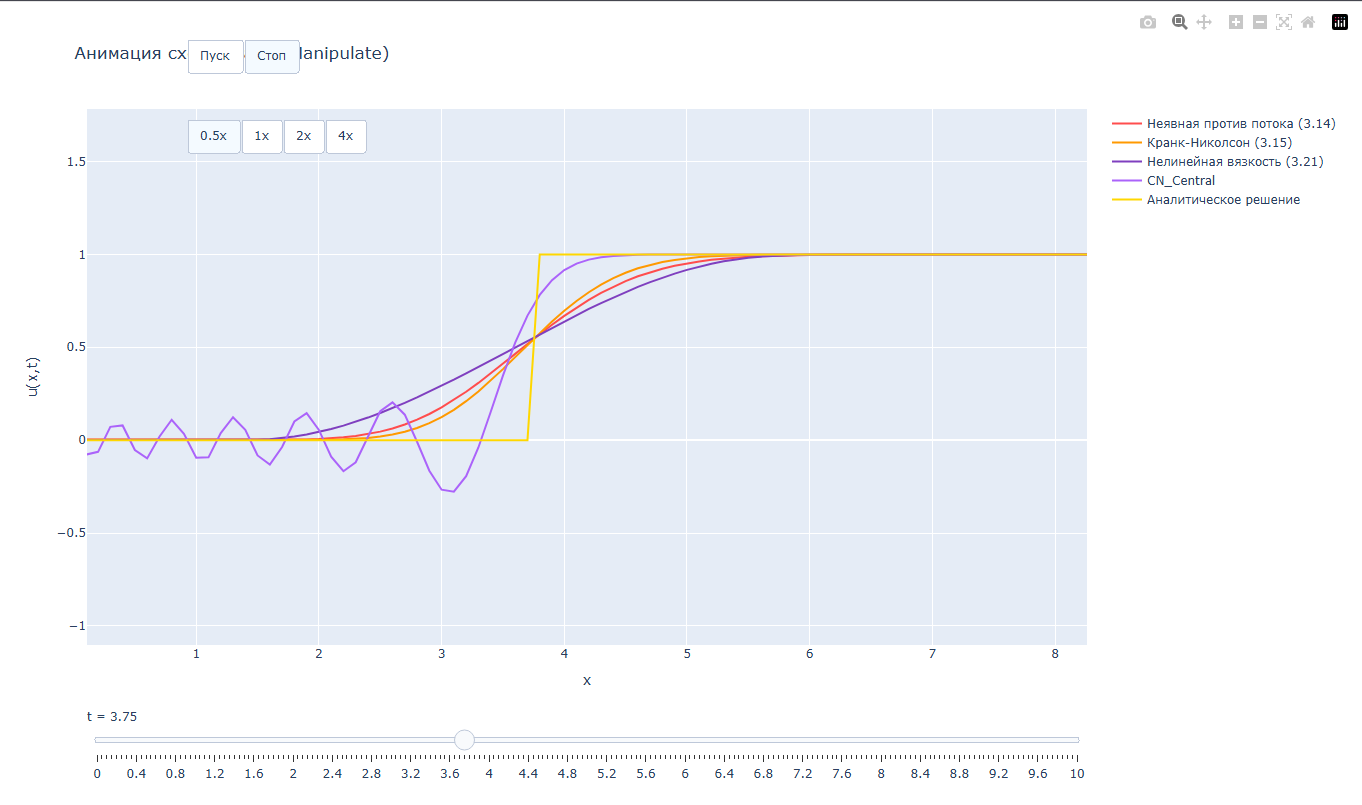
\includegraphics[width=0.9\linewidth]{image_2026-04-25_16-55-57.png}
	\caption{}
	\label{fig:image2026-04-2516-55-57}
\end{figure}


 Благодаря этому весь остальной интерфейс --- графики, таблицы ошибок, анализ сходимости --- не зависит от того, каким способом было получено решение. Унифицированный формат результата является одним из главных факторов простоты расширения системы.

\sectionc{Расчёт ошибок и анализ сходимости}

Функция расчёта норм принимает численное и аналитическое решения, а также пространственный шаг. Для каждого временного слоя вычисляются нормы $L_1$, $L_2$ и $L_\infty$, показанных на рисунке \eqref{fig:image2026-04-2517-02-06}

\begin{figure}[H]
	\centering
	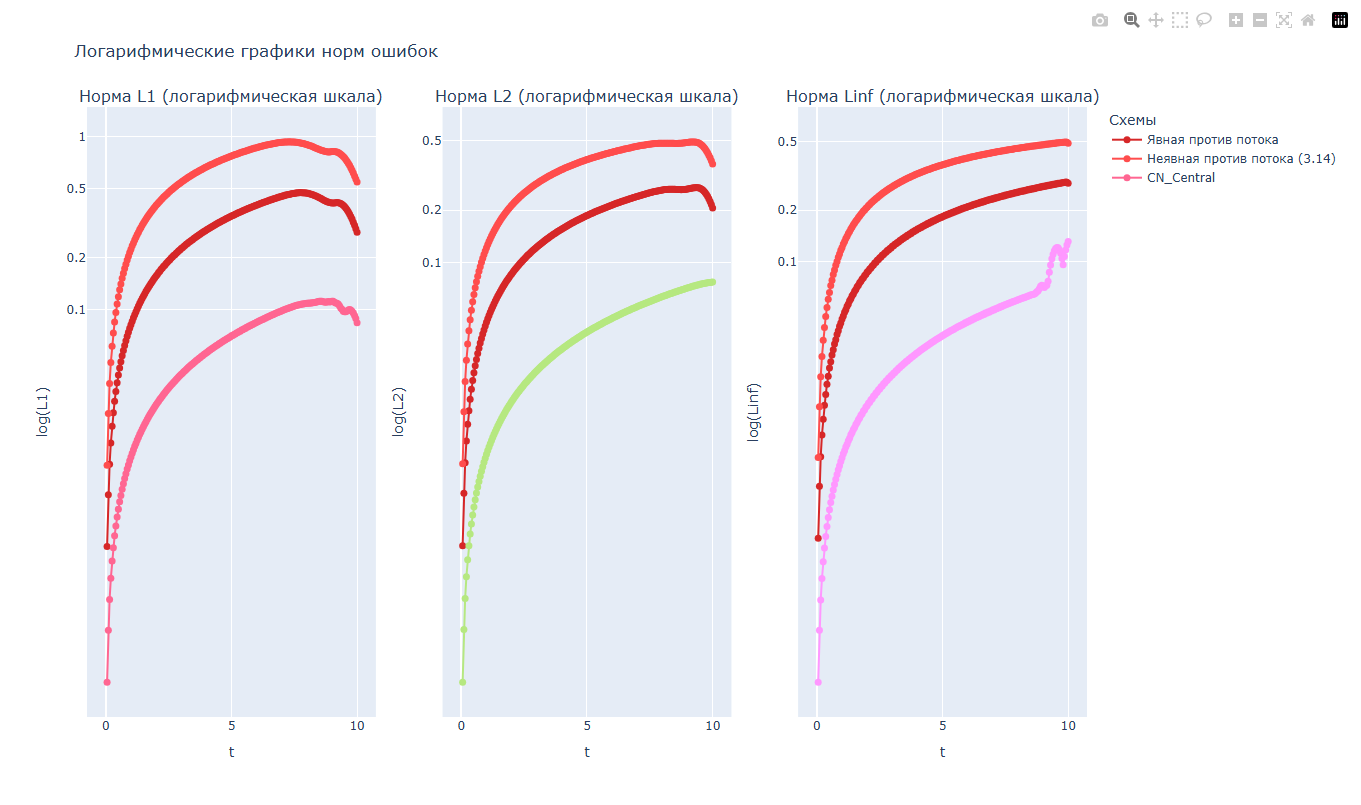
\includegraphics[width=0.9\linewidth]{image_2026-04-25_17-02-06.png}
	\caption{}
	\label{fig:image2026-04-2517-02-06}
\end{figure}
Далее результаты используются в нескольких сценариях:

\begin{itemize}
    \item построение графиков динамики норм во времени;
    \item формирование итоговой сравнительной таблицы;
    \item сортировка схем по величине ошибки на последнем шаге;
    \item отображение текстового отчёта в интерфейсе.
\end{itemize}

Анализ сходимости реализован как серия расчётов одной выбранной схемы на последовательности сеток. Пользователь выбирает ровно один метод, после чего программа несколько раз строит решение при разных значениях $N_x$, вычисляет итоговую ошибку в норме $L_2$ и формирует логарифмический график зависимости ошибки от шага $h$. Такая процедура позволяет экспериментально оценить порядок сходимости и проверить, согласуется ли он с теоретическими ожиданиями. Пример на рисунке \eqref{fig:image2026-04-2517-06-12}

\begin{figure}[H]
	\centering
	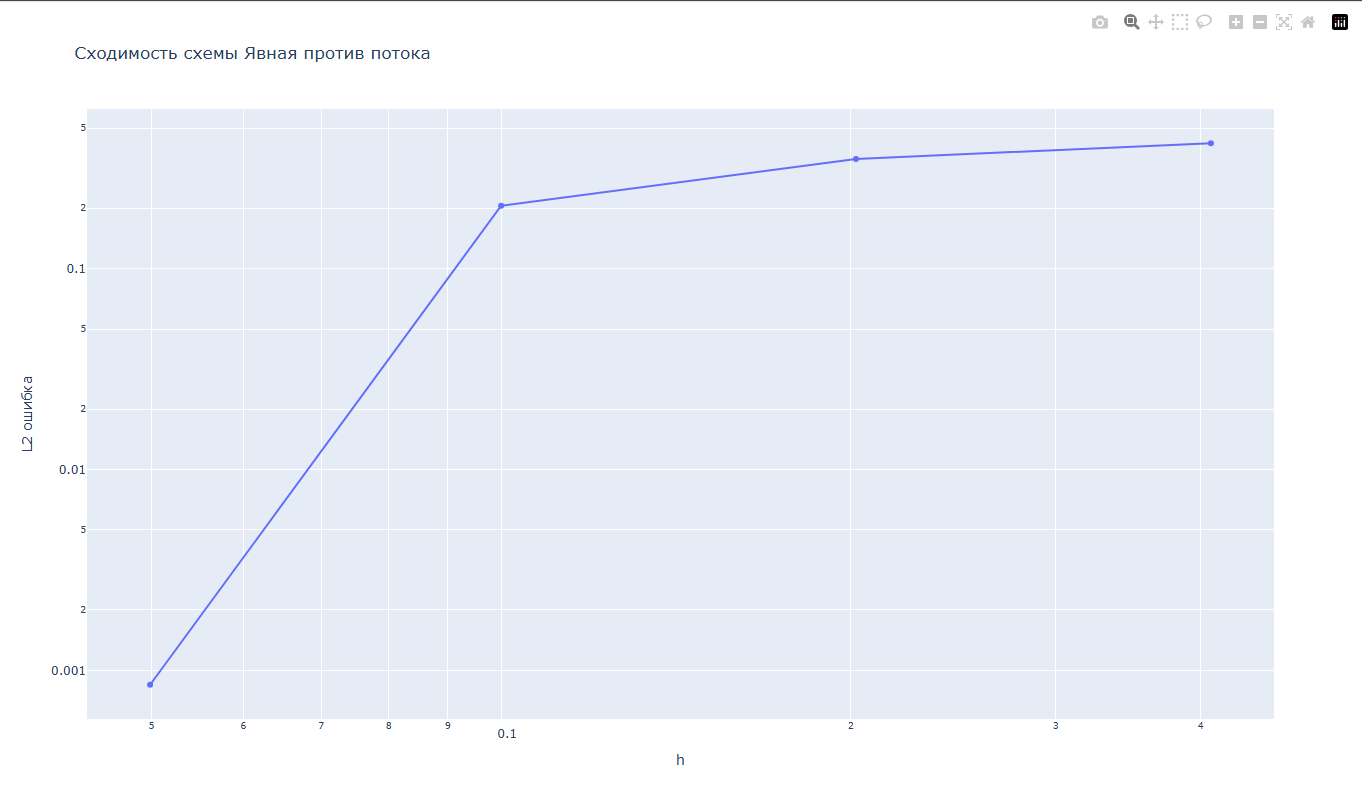
\includegraphics[width=0.7\linewidth]{image_2026-04-25_17-06-12.png}
	\caption{}
	\label{fig:image2026-04-2517-06-12}
\end{figure}

С точки зрения инженерии важно, что реализация анализа сходимости использует уже существующие функции контекста и схем. Это означает, что соответствующая функциональность появилась не за счёт дублирования кода, а благодаря повторному использованию базовых модулей. Подобный результат подтверждает правильность выбранной архитектуры.

\sectionc{Визуализация и экспорт}

В приложении реализовано несколько типов визуализации. Анимация сравнения схем показывает эволюцию профиля во времени и содержит кнопки запуска, остановки и изменения скорости воспроизведения. Режим среза позволяет сравнить решения в фиксированный момент времени. Дополнительно доступны контурный график и трёхмерная поверхность аналитического решения, а также отображение характеристик.

Наличие нескольких представлений одной и той же информации имеет не декоративный, а методический смысл. Линейный график позволяет сопоставить формы профилей, контурное изображение показывает общую картину переноса, а трёхмерная поверхность подчёркивает связь между пространством, временем и значением решения. Визуализация характеристик особенно полезна при обсуждении физического смысла задачи и происхождения аналитической формулы.

Экспорт анимации реализован через отдельный рабочий объект, помещаемый в поток \texttt{QThread}. Это решение предотвращает блокировку пользовательского интерфейса при длительном формировании кадров. Пользователь видит окно прогресса, может отменить операцию и получает текстовый отчёт о результате. Подобная организация долгих операций является хорошей практикой разработки настольных приложений.


\chapter{Результаты вычислительных экспериментов}

\sectionc{Организация экспериментов}

Для проверки работоспособности и полезности приложения были выполнены серии вычислительных экспериментов. В качестве базового начального условия часто использовалась функция

\begin{equation}
    \varphi_0(x)=\exp(-x^2),
\end{equation}

поскольку она одновременно достаточно гладкая, хорошо визуализируется и позволяет наблюдать как чистое смещение профиля, так и эффекты численного размывания или осцилляций. В отдельных экспериментах рассматривались и более сложные пользовательские выражения, в том числе с использованием ступенчатых функций:

\begin{equation}
	\varphi_0(x) = \theta(x),
\end{equation}

Для пространственно-временной области использовались диапазоны, позволяющие видеть динамику решения на интервале, где профиль не успевает полностью выйти за пределы области наблюдения. Плотность сетки варьировалась от умеренной до повышенной, чтобы проследить влияние шагов $h$ и $\tau$ на ошибку и устойчивость. Отдельно оценивался эффект изменения числа узлов при фиксированной постановке задачи для анализа сходимости.

\sectionc{Сравнение явных схем}

Наиболее показательные различия между методами проявляются при сравнении явной схемы против потока, схем Лакса -- Фридрихса и Лакса -- Вендроффа(рисунок \eqref{fig:image2026-04-2517-15-17}).

\begin{figure}[H]
	\centering
	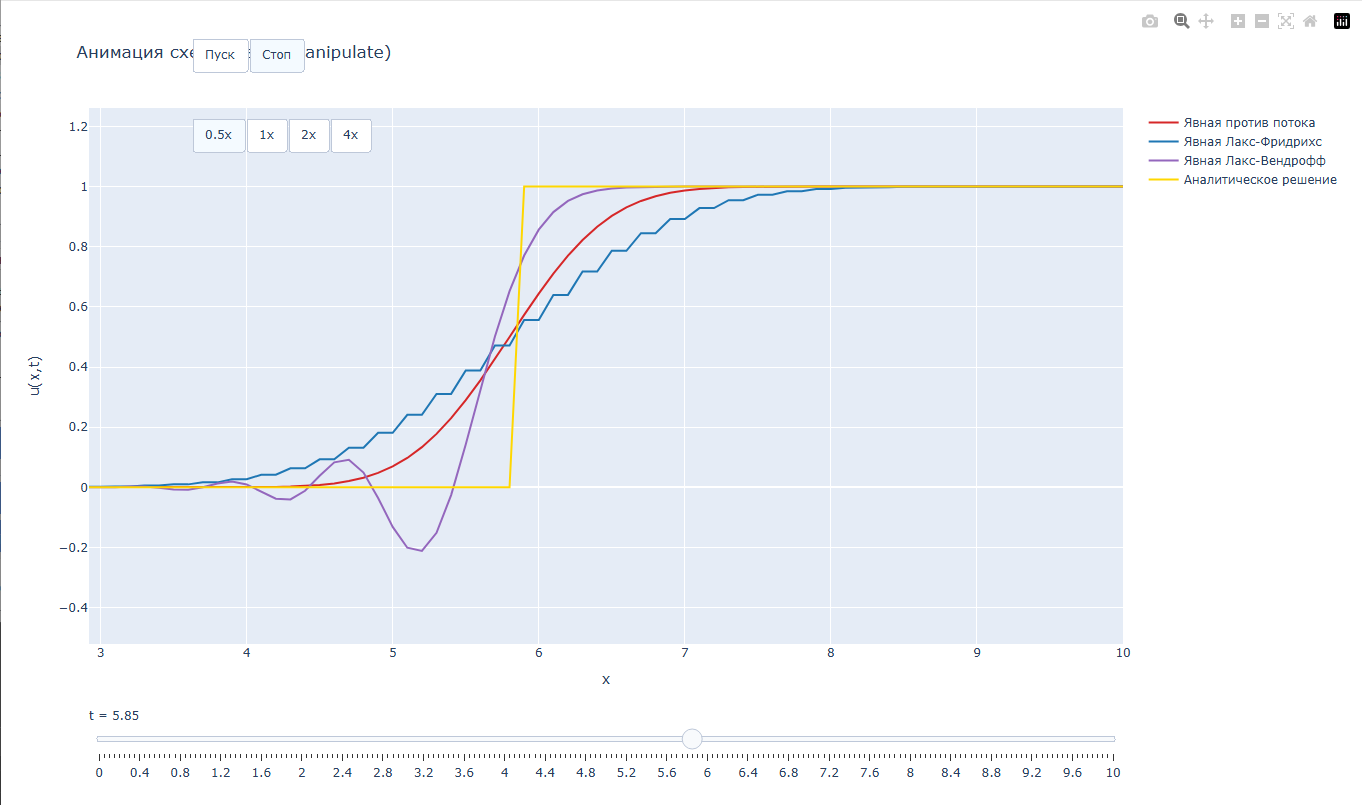
\includegraphics[width=0.9\linewidth]{image_2026-04-25_17-15-17.png}
	\caption{}
	\label{fig:image2026-04-2517-15-17}
\end{figure}


 Апвиндный метод, как и ожидалось, демонстрирует устойчивое, но более размытое решение. При длительном переносе гладкий максимум профиля постепенно уплощается, а фронты сглаживаются. Этот эффект хорошо соответствует представлению о численной вязкости.

Схема Лакса--Фридрихса также проявляет заметную диссипацию. В ряде сценариев она оказывается даже более сглаживающей, чем апвиндная схема, хотя и остаётся полезной как простой эталонный метод. Схема Лакса--Вендроффа, напротив, лучше сохраняет форму гладкого профиля, но при недостаточно аккуратном выборе параметров может порождать волнообразные артефакты. Именно поэтому включение в приложение сразу нескольких схем оказывается методически оправданным: пользователь наблюдает не абстрактные рассуждения о порядке точности, а конкретные различия на одном и том же графике.

Схема Мак-Кормака занимает промежуточное положение и демонстрирует хороший баланс между точностью и наглядностью. В учебном контексте она удобна ещё и тем, что двухшаговая структура предиктор--корректор легко объясняется и визуально связывается с получаемым результатом.

\sectionc{Роль ограничителей и схем TVD/MUSCL}

При использовании ограничителей minmod и MC удалось продемонстрировать важный для гиперболических задач эффект: уменьшение паразитических колебаний без катастрофического роста диссипации. На гладких профилях TVD- и MUSCL-схемы дают более аккуратное решение по сравнению с простыми центральными подходами(\eqref{fig:image2026-04-2516-49-52}), а на крутых фронтах ведут себя устойчивее.

Визуально различие между ограничителями можно описать так: minmod обеспечивает более строгую монотонность, но в ряде случаев сильнее сглаживает локальные особенности, тогда как MC допускает более точное восстановление наклона и лучше сохраняет форму, если решение остаётся достаточно гладким. Возможность сравнить эти варианты в едином интерфейсе полезна не только для обучения, но и для подготовки к исследовательской части выпускной квалификационной работы.

\sectionc{Сравнение неявных схем}

Неявные методы (рисунок \eqref{fig:image2026-04-2516-55-57}) оказались особенно интересны в ситуациях, где явные схемы чувствительны к размеру временного шага. При увеличении $\tau$ устойчивость неявных схем сохраняется лучше, что подтверждает теоретические ожидания. При этом наблюдаются отличия по диссипативным свойствам: одни схемы сохраняют профиль сравнительно хорошо, другие дают более сглаженный результат, но при этом остаются стабильными.

Практически значимым оказался режим сравнения неявной центральной схемы, варианта Кранка--Николсона и методов с искусственной вязкостью. Кранк--Николсон демонстрирует высокий интерес как компромиссный подход: он даёт хорошую точность, но при этом требует решения системы на каждом временном шаге. Схемы с регуляризацией и дополнительной вязкостью полезны для исследования влияния стабилизирующих членов на итоговую ошибку.

\sectionc{Пользовательские схемы как инструмент исследования}

Особый класс экспериментов связан с пользовательскими схемами. В конфигурационном файле приложения были подготовлены примеры пользовательской явной схемы, центральной формулы и нескольких матричных модификаций по типу Кранка--Николсона. Эти примеры подтвердили работоспособность формата хранения и механизма загрузки: приложение корректно интерпретирует пользовательское описание, включает схему в общий список и позволяет анализировать её наравне со встроенными методами.

С методической точки зрения это одна из наиболее сильных сторон проекта. Пользователь может не только выбрать готовую схему, но и воспроизвести литературный метод по формуле из учебника или статьи. Если схема оказывается неустойчивой либо выдаёт большую ошибку, это тоже полезный результат, поскольку он непосредственно демонстрирует последствия неудачного выбора аппроксимации.

\sectionc{Анализ ошибок и таблицы норм}

Расчёт норм ошибок показал, что итоговая оценка метода зависит от выбранной метрики. Для гладких начальных данных схемы второго порядка закономерно демонстрируют меньшие значения $L_2$ и $L_1$ при достаточном разрешении сетки. Однако в норме $L_\infty$ на отдельных сценариях более строгие методы с ограничителями выглядят предпочтительнее из-за меньшей амплитуды локальных выбросов.

Наличие таблицы итоговых ошибок в интерфейсе оказалось очень полезным. Когда пользователь сравнивает сразу несколько схем, график даёт качественное представление, а таблица --- количественное. Совместное использование этих форм представления результатов является важным достоинством разработанного приложения.

\sectionc{Анализ сходимости}

При последовательном уточнении сетки приложение строит логарифмический график зависимости ошибки в норме $L_2$ от шага $h$. Такой график позволяет визуально оценить скорость убывания ошибки и, следовательно, экспериментально судить о порядке сходимости. Хотя в учебных условиях на конечных сетках нельзя ожидать идеального совпадения с асимптотической теорией, получаемые кривые демонстрируют качественно правильное поведение: схемы более высокого порядка показывают более быстрое снижение ошибки в зоне, где доминирует именно аппроксимационная составляющая.

Важным наблюдением является то, что порядок сходимости может искажаться при слишком грубых сетках, слишком большом числе Куранта или недостаточно гладком начальном условии. Следовательно, анализ сходимости в приложении полезен не только как подтверждение теории, но и как инструмент обсуждения ограничений самой теории при практическом вычислительном эксперименте.

\sectionc{Интерпретация результатов с точки зрения учебного процесса}

Проведённые эксперименты показывают, что приложение действительно выполняет функцию интерактивной учебной лаборатории. Оно позволяет переходить от абстрактных формул к непосредственному наблюдению поведения схем, а также быстро изменять параметры и получать новый результат. Для преподавателя это средство демонстрации, для студента --- инструмент самостоятельного эксперимента, а для разработчика выпускной квалификационной работы --- удобная база для последующих расширений.

Именно сочетание количественного анализа, визуализации и пользовательской расширяемости делает результат практики содержательно завершённым. Без визуализации продукт был бы просто вычислительным скриптом, без анализа ошибок --- красивой, но слабо полезной оболочкой, а без поддержки пользовательских схем --- закрытым демонстратором. Совместная реализация всех трёх составляющих обеспечивает целостность разработанной системы.

\chapter{Тестирование, отладка и оценка качества}

\sectionc{Стратегия тестирования}

Тестирование приложения проводилось на нескольких уровнях. На уровне входных данных проверялась корректность обработки числовых параметров, выражений для коэффициента переноса и начального условия, а также ситуаций с недопустимыми диапазонами по пространству и времени. На уровне вычислительных функций оценивалась способность схем возвращать массивы согласованных размеров, корректно обрабатывать границы и выдавать осмысленные ошибки при нарушении условий применимости.

На уровне сценариев пользовательского интерфейса проверялись основные действия: выбор режимов, расчёт анимации, построение срезов, вычисление норм, анализ сходимости, добавление и удаление пользовательских схем, экспорт результатов. Особое внимание уделялось сценариям, где потенциально возможна потеря управления интерфейсом, например при длительном экспорте анимации. Для таких случаев был реализован отдельный поток и окно прогресса.

\sectionc{Тестовые сценарии}

\begin{longtable}{p{0.1\textwidth}p{0.33\textwidth}p{0.42\textwidth}} 
Тест & Описание & Ожидаемый результат \\
T1 & Ввод некорректного числа в поле границы сетки & Появляется сообщение об ошибке, программа не завершается аварийно. \\
T2 & Задание $x_{\max} \le x_{\min}$ & Пользователь получает уведомление о некорректной области. \\
T3 & Выбор аналитического режима для $a=a(x)$ с нулями коэффициента на сетке & Система сообщает, что коэффициент недопустим для такого режима. \\
T4 & Построение анимации для набора встроенных схем & Открывается интерактивная анимация с ползунком времени. \\
T5 & Расчёт норм ошибок для нескольких схем & Строятся графики норм и открывается таблица итоговых значений. \\
T6 & Анализ сходимости без выбора схемы или при выборе нескольких схем & Отображается сообщение о необходимости выбрать ровно одну схему. \\
T7 & Добавление пользовательской явной схемы & Схема появляется в списке и может участвовать в расчётах. \\
T8 & Экспорт анимации в GIF или MP4 & Создаётся файл результата, интерфейс остаётся отзывчивым. \\
T9 & Отмена экспорта пользователем & Операция прекращается без зависания и без некорректных остаточных файлов. \\
\end{longtable}

Указанные сценарии подтвердили, что система в целом устойчива к типовым ошибкам пользователя и обеспечивает воспроизводимую работу в основном наборе задач. Разумеется, проект остаётся расширяемым, и его можно дополнительно покрыть автоматическими модульными тестами, однако для задач преддипломной практики полученный уровень надёжности можно считать достаточным.

\sectionc{Анализ производительности}

Основная вычислительная нагрузка в приложении связана с временными циклами по сетке и построением анимаций. Для умеренных размеров сетки производительность Python с использованием NumPy оказывается достаточной. Явные схемы работают быстро, а неявные методы демонстрируют приемлемую скорость даже при необходимости решать линейную систему на каждом временном шаге, поскольку используются специализированные методы для ленточных матриц.

Более тяжёлой операцией является экспорт анимации. Здесь значительную роль играют не столько сами вычисления решения, сколько отрисовка кадров и кодирование итогового файла. Именно поэтому было принято решение выполнять экспорт в отдельном потоке. С точки зрения пользовательского опыта такое решение является критически важным: даже если операция занимает заметное время, пользователь сохраняет контроль над программой и может её отменить.

\sectionc{Ограничения текущей версии}

Несмотря на достигнутый результат, текущая версия системы имеет ряд ограничений. Во-первых, приложение ориентировано на одномерное уравнение переноса и не рассматривает двумерные задачи. Во-вторых, для некоторых аналитических режимов требуется выполнение условий монотонности и ненулевого коэффициента. В-третьих, пользовательские схемы интерпретируются через выражения, что требует аккуратности при валидации и ограничивает набор поддерживаемых конструкций безопасным вычислительным контуром. Кроме того, проект в основном ориентирован на интерактивное исследование, а не на пакетные вычисления. Если в будущем потребуется запуск больших серий экспериментов без графического интерфейса, будет целесообразно выделить вычислительное ядро в отдельный модуль с командной строкой или API.

\chapter{Практические результаты и сформированные компетенции}

Преддипломная практика позволила получить не только программный продукт, но и набор профессиональных результатов, непосредственно связанных с подготовкой выпускной квалификационной работы. К основным практическим результатам можно отнести:

\begin{itemize}
    \item разработку настольного приложения, решающего прикладную задачу исследования уравнения переноса;
    \item реализацию набора явных и неявных численных схем в единой архитектуре;
    \item внедрение аналитического эталона для ряда модельных случаев;
    \item создание механизма добавления пользовательских схем без изменения исходного кода;
    \item реализацию средств анализа ошибок, сходимости и устойчивости;
    \item подготовку отчётной документации, пригодной для дальнейшего использования в дипломном проекте.
\end{itemize}

С точки зрения профессиональных компетенций практика способствовала развитию способности:

\begin{enumerate}
    \item формализовать прикладную задачу в виде математической модели;
    \item выбирать адекватные численные методы и обосновывать их свойства;
    \item проектировать структуру программной системы с учётом расширяемости;
    \item реализовывать графические интерфейсы для научных приложений;
    \item проводить вычислительный эксперимент и интерпретировать его результаты;
    \item оформлять результаты работы в виде технической и отчётной документации.
\end{enumerate}

Важным итогом стало понимание того, что качественный научно-образовательный программный продукт определяется не только корректностью алгоритмов, но и тем, насколько удобно пользователь может провести полный цикл исследования: ввести данные, получить результат, сравнить методы, зафиксировать выводы и воспроизвести эксперимент. Именно в таком комплексном виде задача была решена в рамках практики.

\chapter{Перспективы развития проекта}

Разработанное приложение имеет хорошие перспективы расширения. Прежде всего возможно развитие математической части. В проект можно добавить задачи с источниковым членом, нелинейные уравнения первого порядка, системы гиперболических уравнений, двумерные постановки и методы конечных объёмов. Это сделает платформу более универсальной и приблизит её к задачам реального инженерного моделирования.

С точки зрения программной архитектуры перспективным направлением является выделение вычислительного ядра в самостоятельный пакет с модульными тестами и документацией API. Тогда графический интерфейс станет лишь одним из способов взаимодействия с вычислительным модулем, а сами расчёты можно будет использовать в командной строке, в Jupyter-ноутбуках или в веб-приложении.

Полезным развитием могло бы стать внедрение системы сохранения и загрузки полных сценариев эксперимента, включающих не только пользовательские схемы, но и все параметры сетки, тип коэффициента, набор выбранных методов и параметры визуализации. Это ещё сильнее повысит воспроизводимость учебных и исследовательских работ.

Наконец, в перспективе можно добавить автоматизированную оценку порядка сходимости, экспорт таблиц ошибок в CSV или Excel, формирование отчётов в PDF по готовому шаблону и более строгую систему валидации пользовательских формул. Все эти направления логично продолжают уже реализованную архитектуру и могут лечь в основу дальнейшей выпускной квалификационной работы.

\chapter*{Заключение}
\addcontentsline{toc}{chapter}{Заключение}

В ходе преддипломной практики была решена комплексная задача разработки настольного приложения для исследования численных схем решения одномерного уравнения переноса. Выполненная работа объединила математический анализ, алгоритмизацию, проектирование архитектуры, разработку графического интерфейса, визуализацию результатов и подготовку итоговой документации. На практике это означало переход от теоретической постановки задачи к созданию реального инструмента, пригодного для учебно-исследовательского использования.

Созданное приложение обеспечивает построение аналитического решения для ряда модельных случаев, поддерживает широкий набор встроенных явных и неявных схем, позволяет пользователю добавлять собственные методы, вычисляет нормы ошибок, оценивает число CFL, строит графики сходимости и экспортирует анимации. Существенным достоинством проекта является то, что все перечисленные возможности объединены в одном интерфейсе и работают в рамках согласованной архитектуры.

Полученный результат имеет как практическую, так и методическую ценность. С одной стороны, разработанная система может служить лабораторной платформой для изучения вычислительных методов. С другой стороны, проект формирует прочную основу для дальнейшей дипломной разработки, в том числе для расширения постановки задачи и углубления математической части. Следовательно, цель преддипломной практики достигнута, а поставленные задачи решены в полном объёме.

\chapter*{Список использованных источников}
\addcontentsline{toc}{chapter}{Список использованных источников}

\begin{enumerate}
    \item Самарский А. А. Теория разностных схем. М.: Наука, 1989.
    \item Годунов С. К., Рябенький В. С. Разностные схемы. М.: Наука, 1977.
    \item LeVeque R. J. Numerical Methods for Conservation Laws. Basel: Birkhauser, 1992.
    \item LeVeque R. J. Finite Volume Methods for Hyperbolic Problems. Cambridge: Cambridge University Press, 2002.
    \item Richtmyer R. D., Morton K. W. Difference Methods for Initial-Value Problems. New York: Interscience Publishers, 1967.
    \item Танненбаум Э., Поллард Г. Обыкновенные дифференциальные уравнения. М.: Мир, 1988.
    \item NumPy Developers. NumPy Documentation. URL: \url{https://numpy.org/doc/}.
    \item SciPy Developers. SciPy Documentation. URL: \url{https://docs.scipy.org/doc/scipy/}.
    \item SymPy Development Team. SymPy Documentation. URL: \url{https://docs.sympy.org/}.
    \item Riverbank Computing. PyQt5 Reference Guide. URL: \url{https://www.riverbankcomputing.com/static/Docs/PyQt5/}.
    \item Qt Company. Qt Documentation. URL: \url{https://doc.qt.io/}.
    \item Plotly Technologies Inc. Plotly Python Documentation. URL: \url{https://plotly.com/python/}.
    \item Sweby P. K. High Resolution Schemes Using Flux Limiters for Hyperbolic Conservation Laws // SIAM Journal on Numerical Analysis. 1984. Vol. 21. No. 5. P. 995--1011.
    \item Toro E. F. Riemann Solvers and Numerical Methods for Fluid Dynamics. Berlin: Springer, 2009.
\end{enumerate}

\appendix

\chapter{Руководство пользователя}

Данное приложение ориентировано на интерактивную работу, поэтому ниже приведён рекомендуемый порядок использования системы.

\sectionc{Запуск программы}

После установки зависимостей приложение запускается как обычный Python-скрипт. Пользователь открывает главное окно, в котором доступны все основные режимы работы. При первом запуске список пользовательских схем загружается из конфигурационного JSON-файла, если такой файл уже был создан ранее.

\sectionc{Базовый сценарий работы}

\begin{enumerate}
    \item Выбрать тип коэффициента переноса в выпадающем списке.
    \item При необходимости ввести аналитическую формулу коэффициента или параметры каталожного случая.
    \item Ввести начальное условие $\varphi_0(x)$.
    \item Задать границы и плотность пространственно-временной сетки.
    \item Отметить интересующие встроенные и пользовательские схемы.
    \item При необходимости включить отображение аналитического решения.
    \item Нажать кнопку нужного режима анализа: анимация, срез, нормы ошибок, итоговые ошибки, сходимость и т.д.
\end{enumerate}

\sectionc{Добавление пользовательской схемы}

Для добавления новой схемы необходимо открыть диалоговое окно по кнопке добавления пользовательской схемы. Затем требуется:

\begin{enumerate}
    \item ввести имя схемы;
    \item выбрать тип реализации;
    \item задать формулу явного перехода либо параметры неявной матрицы;
    \item сохранить схему;
    \item отметить её флажком в основном окне для участия в сравнении.
\end{enumerate}

Пользовательские схемы сохраняются в JSON-файл и доступны при следующих запусках программы. Это особенно удобно при подготовке лабораторных работ и дипломных материалов, когда один и тот же набор методов используется многократно.

\sectionc{Интерпретация результатов}

При анализе результатов рекомендуется учитывать несколько факторов одновременно:

\begin{itemize}
    \item форму графика и наличие видимых осцилляций;
    \item значение норм ошибок и их динамику во времени;
    \item величину CFL-числа;
    \item влияние сгущения сетки на итоговую точность;
    \item различия между гладкими и негладкими начальными условиями.
\end{itemize}

Именно комплексный подход позволяет сделать корректный вывод о качестве численной схемы. Одна только визуализация или одна только таблица ошибок дают неполную картину.

\chapter{Каталог реализованных схем}

\sectionc{Встроенные явные схемы}

\begin{longtable}{p{0.3\textwidth}p{0.25\textwidth}p{0.33\textwidth}}
Схема & Класс метода & Краткая характеристика \\
Явная против потока & Апвиндная & Проста, устойчива при допустимом CFL, обладает численной вязкостью. \\
Явная Лакс--Фридрихс & Центральная с усреднением & Надёжна, но заметно сглаживает решение. \\
Явная Лакс--Вендрофф & Второй порядок & Лучше сохраняет гладкие профили, может осциллировать. \\
Явная вязкость & Стабилизированная & Добавляет искусственную вязкость, подавляет колебания. \\
Явная Мак-Кормак & Предиктор--корректор & Точна на гладких решениях, наглядна методически. \\
Явная TVD (minmod) & TVD & Подавляет осцилляции, более диссипативна. \\
Явная MUSCL (MC) & TVD/MUSCL & Сохраняет форму лучше minmod, требует аккуратной интерпретации. \\
Явная Русанов & Потоковая & Использует апвиндный поток, устойчива и проста. \\
Явная Годунов & Потоковая & Близка к апвиндной логике для данного класса задач. \\
\end{longtable}

\sectionc{Встроенные неявные схемы}

\begin{longtable}{p{0.3\textwidth}p{0.25\textwidth}p{0.33\textwidth}}
Схема & Тип матрицы & Назначение \\
Неявная против потока (3.14) & Трёхдиагональная & Базовый неявный апвиндный метод. \\
Неявная центральная gen & Трёхдиагональная & Центральная аппроксимация для исследования устойчивости. \\
Неявная Лакс--Вендрофф (3.19) & Трёхдиагональная & Неявный аналог схемы повышенного порядка. \\
Кранк--Николсон (3.15) & Трёхдиагональная & Компромисс между точностью и устойчивостью. \\
Неявная апвинд (3.17) & Трёхдиагональная & Направленная схема с учётом знака скорости. \\
Линейная вязкость (3.20) & Трёхдиагональная & Стабилизация за счёт вязкостного члена. \\
Вязкость 4-го порядка (3.18) & Пентадиагональная & Более сложная регуляризация. \\
Нелинейная вязкость (3.21) & Трёхдиагональная & Коэффициент вязкости зависит от локального решения. \\
Регуляриз. Лакс--Вендрофф (3.19) & Трёхдиагональная & Комбинирует точность и стабилизацию. \\
\end{longtable}

\chapter{Фрагменты конфигурации и кода}

В приложении пользовательские схемы сохраняются в JSON-представлении. Ниже приведён иллюстративный пример такого описания. Для совместимости с pdf\LaTeX{} в листинге использованы ASCII-метки типов; в рабочем файле проекта допускаются и русскоязычные обозначения.

\begin{lstlisting}[language={},caption={Пример пользовательской конфигурации схем}]
{
    "upwind_custom": [
        "u - a * dt / dx * (u - u_left)",
        "explicit"
    ],
    "Matrix_Crank_Nicolson": [
        {
            "diagonals": {
                "0": "1",
                "-1": "-a * dt / (2 * dx)",
                "1": "a * dt / (2 * dx)"
            },
            "rhs": "u - a * dt / (2 * dx) * (u_right - u_left)"
        },
        "implicit_matrix"
    ]
}
\end{lstlisting}

Такая форма хранения делает расширение приложения прозрачным для пользователя. Система читает конфигурацию, нормализует описание схемы и подключает её к общему вычислительному контуру. При необходимости список может быть дополнен новыми записями через графический интерфейс.

Ещё один показательный фрагмент связан с вычислением числа CFL:

\begin{lstlisting}[language=Python,caption={Расчёт числа Куранта в приложении}]
dx, dt = dxdt(ctx)
xg, tg = np.meshgrid(ctx.x, ctx.t, indexing="xy")
a_max = np.max(np.abs(ctx.a(xg, tg)))
cfl = a_max * dt / dx
\end{lstlisting}

Несмотря на краткость, данный код играет важную роль в пользовательском сценарии: он связывает математическое требование устойчивости с конкретными параметрами сетки и режима коэффициента переноса.

\end{document}